\documentclass{beamer}
\usepackage{amsmath}
\usepackage[english, russian]{babel}
\usepackage{bbm}
\usepackage{graphicx}
\usepackage[T2A, T1]{fontenc}
\usepackage[utf8]{inputenc}
\usepackage{tikz}
\usepackage{wrapfig}

\usetikzlibrary{shapes,arrows}
\tikzstyle{block} = [rectangle, draw,% fill=blue!20, 
    text width=10em, text centered, rounded corners]%, minimum height=4em]
\tikzstyle{line} = [draw, -latex']

\mode<presentation>
\usetheme{Warsaw}

\bibliographystyle{unsrt}


\title{Краевые моды и связанные состояния в топологических изоляторах}
\author[Е. Аникин]{Евгений Аникин \\
	научный руководитель\\
	чл.-к.~РАН~д.~ф--м.~н.~П.И. Арсеев}
\institute{ФИАН им. Лебедева}
\date{}

\begin{document}

\begin{frame}
    \titlepage
\end{frame}

\begin{frame}
    \frametitle{Двумерный топологический изолятор на базе HgTe}
    \begin{itemize}
        \item Отличен от нуля $\mathrm{TKNN}$--инвариант:
            \begin{equation}
                \label{TKNN}
                N = \frac{1}{2\pi i} 
                    \int d^2 k\, \left(\partial_x \langle u | \partial_y u \rangle -
                    \partial_y \langle u | \partial_x u \rangle \right)
            \end{equation}
        \item Невозможно задать функцию Блоха во всей зоне Бриллюэна
        \item Есть киральные краевые состояния
    \end{itemize}
\end{frame}

\begin{frame}
    \frametitle{Пример топологического изолятора}
        Эффективный гамильтониан для E1, H1 подуровней квантовой ямы HgTe:
        \begin{equation}
           \label{eff_so_ham}
            \scalebox{0.6}{%
            $
            H = \left(\begin{matrix}
                    \xi + \frac{1}{m}(2 - \cos{p_x} - \cos{p_y}) & 
                            2t(\sin{p_x} - i\sin{p_y})   \\
                    2t(\sin{p_x} + i\sin{p_y}) & 
                           - \xi - \frac{1}{m}(2 - \cos{p_x} - \cos{p_y}) \\
                \end{matrix}\right)
            $
            }
        \end{equation}
        Описывает топологический изолятор при $\xi < 0$
\end{frame}

\begin{frame}
    \begin{columns}
        \frametitle{Защищённость краевых состояний}
        \begin{column}{0.5\textwidth}
            \begin{tikzpicture}[node distance = 2cm, auto]
                \node [block] (first) {ветви краевых состояний образуют крамерсовский дублет};
                \node [block, below of=first] (second){нет рассеяния};
                \path [line] (first) -- (second);
            \end{tikzpicture}
        \end{column}
        \begin{column}{0.5\textwidth}
            \begin{figure}
                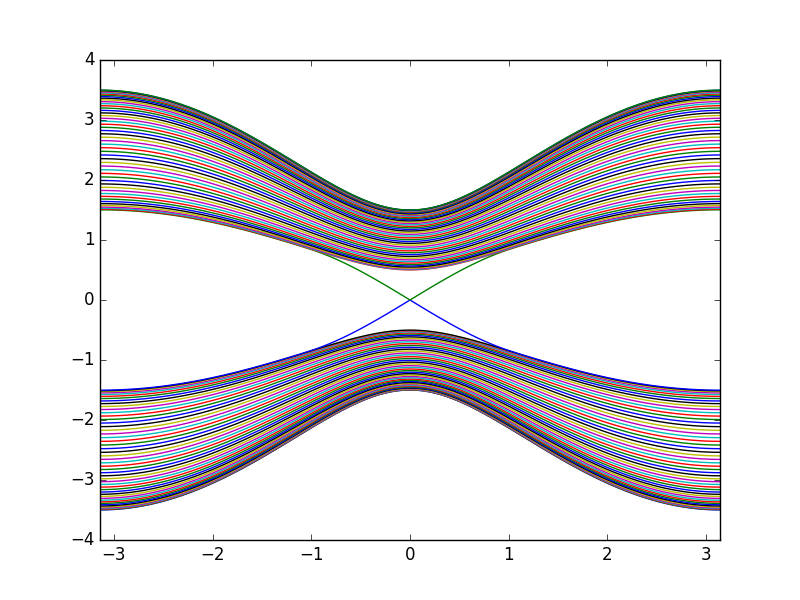
\includegraphics[width=\linewidth]{eff_ham_stripe.png}
                \caption{Спектр полосы конечной толщины}
            \end{figure}
        \end{column}
    \end{columns}
\end{frame}

\begin{frame}
    \frametitle{Спин--орбитальное взаимодействие в подходе сильной связи}
    \textbf{\large Составляющие модели}
    \begin{itemize}
        \item $s$--орбитали зоны проводимости
        \item $p$--орбитали валентной зоны
        \item Перекрытия ближайших соседей $t_\parallel$, $t_\perp$, $m_s$, $P$
        \item Атомное спин--орбитальное взаимодействие
    \end{itemize}
\end{frame}

\begin{frame}
    \frametitle{Спин--орбитальное взаимодействие в подходе сильной связи}
    Атомные $p$--орбитали:
    \begin{columns}
    \begin{column}{0.5\textwidth}
    \begin{equation}
    	\label{transform1}
        \scalebox{0.6}{$
    	\begin{gathered}
            \Psi_{\frac{3}{2},\frac{3}{2}} = \frac{X + iY}{\sqrt{2}}\alpha\\
            \Psi_{\frac{3}{2}, \frac{1}{2}} = \sqrt{\frac{1}{3}}\frac{X + iY}{\sqrt{2}}\beta -
                                             \sqrt{\frac{2}{3}} Z\alpha\\
            \Psi_{\frac{3}{2}, -\frac{1}{2}} = -\sqrt{\frac{1}{3}}\frac{X - iY}{\sqrt{2}}\alpha -
                                             \sqrt{\frac{2}{3}} Z\beta\\
            \Psi_{\frac{3}{2},-\frac{3}{2}} = -\frac{X - iY}{\sqrt{2}}\beta
    	\end{gathered}
        $}
    \end{equation}
    \end{column}
    \begin{column}{0.5\textwidth}
    \begin{equation}
    	\label{transform2}
        \scalebox{0.6}{$
    	\begin{gathered}
            \Psi_{\frac{1}{2}, \frac{1}{2}} = \sqrt{\frac{2}{3}}\frac{X + iY}{\sqrt{2}}\beta +
                                             \sqrt{\frac{1}{3}} Z\alpha\\
            \Psi_{\frac{1}{2}, -\frac{1}{2}} = -\sqrt{\frac{2}{3}}\frac{X - iY}{\sqrt{2}}\alpha-
                                             \sqrt{\frac{1}{3}} Z\beta\\
    	\end{gathered}
        $}
    \end{equation}
    \end{column}
    \end{columns}
\end{frame}

\begin{frame}
    \frametitle{Спин--орбитальное взаимодействие в подходе сильной связи}
    Гамильтониан валентной зоны:
    \begin{equation}
        \scalebox{0.6}{
        $
        \begin{gathered}
        H_v = \begin{bmatrix}
                H_l & H_r
            \end{bmatrix},\\
        H_l = 
        \begin{pmatrix}
            (t_\parallel + t_\perp)(\cos{p_x} + \cos{p_y}) + 2t_\perp \cos{p_z} & 0 \\
            0 & \left(\frac{t_\parallel}{3} + \frac{5t_\perp}{3}\right)(\cos{p_x}+\cos{p_y})+ 
                          \left(\frac{2t_\perp}{3} + \frac{4t_\parallel}{3}\right)\cos{p_z} \\
            -\frac{1}{\sqrt{3}}(t_\parallel - t_\perp)(\cos{p_x} - \cos_{p_y}) & 0 \\
            0 & -\frac{1}{\sqrt{3}}(t_\parallel - t_\perp)(\cos{p_x} - \cos_{p_y}) 
        \end{pmatrix}\\
        H_r = 
        \begin{pmatrix}
            -\frac{1}{\sqrt{3}}(t_\parallel - t_\perp)(\cos{p_x} - \cos_{p_y}) & 0 \\
            0 & -\frac{1}{\sqrt{3}}(t_\parallel - t_\perp)(\cos{p_x} - \cos_{p_y})\\
           \left(\frac{t_\parallel}{3} + \frac{5t_\perp}{3}\right)(\cos{p_x} + \cos{p_y}) + 
                     \left(\frac{2t_\perp}{3} + \frac{4t_\parallel}{3}\right)\cos{p_z} & 0 \\
            0 & (t_\parallel + t_\perp)(\cos{p_x} + \cos{p_y}) + 2t_\perp \cos{p_z}
        \end{pmatrix}
        \end{gathered}
        $
        }
    \end{equation}
\end{frame}
\begin{frame}
    \frametitle{Спин--орбитальное взаимодействие в подходе сильной связи}
    Разложение около нуля:
    \begin{equation}
    H_v = -\left(\gamma_1 + \frac{5}{2}\gamma_2\right) k^2 + 
        2\gamma_2(k_x^2J_x^2 + k_y^2J_y^2 + k_z^2J_z^2),
    \end{equation}
    где $J_i$ --- операторы момента для спина $\frac{3}{2}$, $\gamma_1 = \frac13 t_\parallel$,
    $\gamma_2 = \frac16(t_\parallel - t_\perp)$
\end{frame}
\begin{frame}
    \frametitle{Спин--орбитальное взаимодействие в подходе сильной связи}
    Перекрытие с $s$ -- зоной:
    \begin{equation}
    \scalebox{0.6}{
    $
    T = P\begin{pmatrix}
            -\frac{1}{\sqrt{2}}(\sin{p_x} + i\sin{p_y}) & \sqrt{\frac{2}{3}}\sin{p_z} &
             \frac{1}{\sqrt{6}}(\sin{p_x} - i\sin{p_y}) & 0 \\  
            0 & -\frac{1}{\sqrt{6}}(\sin{p_x} + i\sin{p_y}) & 
            \sqrt{\frac{2}{3}}\sin{p_z} & \frac{1}{\sqrt{2}}(\sin{p_x} - i\sin{p_y}),
         \end{pmatrix},
    $}
    \end{equation}
    где $P = 2i\langle s(x+e_x) | \hat{H} | p_x(x)\rangle$.
\end{frame}
\begin{frame}
    \frametitle{Спин--орбитальное взаимодействие в подходе сильной связи}
    В результате получается модель Кейна.
    \begin{figure}
        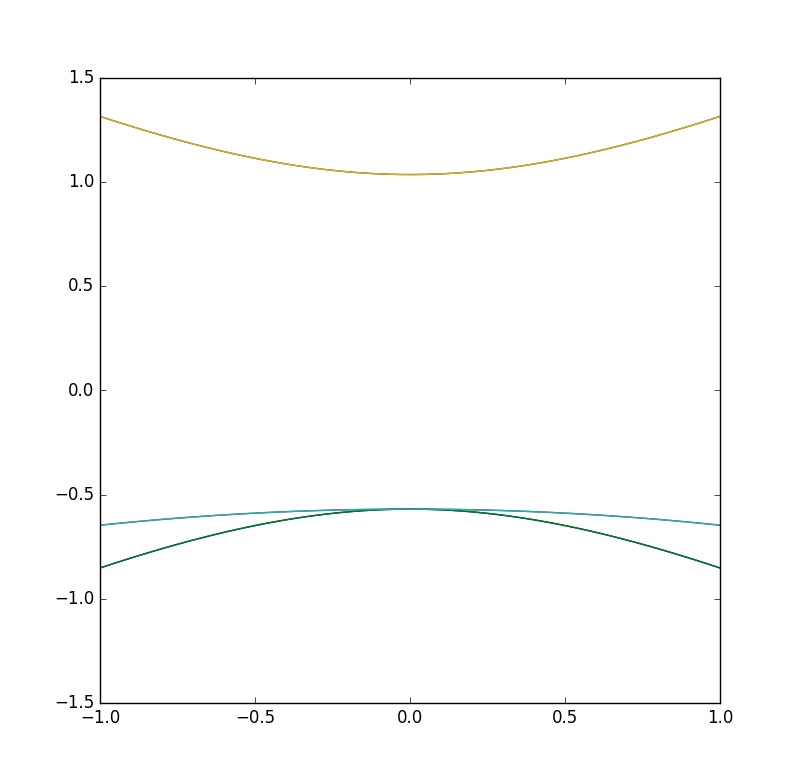
\includegraphics[height=0.6\textheight]{cdte.png}
        \caption{Спектр CdTe}
    \end{figure}
\end{frame}
\begin{frame}
    \frametitle{Упрощённая модель квантовой ямы}
    Полный гамильтониан расщепляется на два блока $3\times 3$.
    \begin{equation}
        \scalebox{0.6}{$
        \label{block}
        H = \begin{pmatrix}
                E_s + \frac{1}{m^*}(2 - \cos{p_x} - \cos{p_y}) &
                -\frac{P}{\sqrt{2}}(\sin{p_x} + i\sin{p_y}) &
                \frac{P}{\sqrt{6}}(\sin{p_x} - i\sin{p_y}) \\
                -\frac{P}{\sqrt{2}}(\sin{p_x} + i\sin{p_y}) &
                (t_\parallel + t_\perp)(\cos{p_x} + \cos{p_y}) &
                -\frac{1}{\sqrt{3}}(t_\parallel - t_\perp)(\cos{p_x} - \cos{p_y}) \\
                \frac{P}{\sqrt{6}}(\sin{p_x} - i\sin{p_y}) &
                -\frac{1}{\sqrt{3}}(t_\parallel - t_\perp)(\cos{p_x} - \cos{p_y}) &
                \left(\frac{t_\parallel}{3} + \frac{5t_\perp}{3}\right)(\cos{p_x} + \cos{p_y})
            \end{pmatrix}
        $}
    \end{equation}
Если $E_s - 2(t_\parallel + t_\perp) \ll \frac{2}{3}(t_\parallel - t_\perp)$,
при малых $k$ ``нижнюю'' дырочную зону можно не учитывать. 
\end{frame}
\begin{frame}
    \frametitle{Пример топологического изолятора}
        Эффективный гамильтониан для E1, H1 подуровней квантовой ямы HgTe:
        \begin{equation}
           \label{eff_so_ham}
            \scalebox{0.6}{%
            $
            H = \left(\begin{matrix}
                    \xi + \frac{1}{m}(2 - \cos{p_x} - \cos{p_y}) & 
                            2t(\sin{p_x} - i\sin{p_y})   \\
                    2t(\sin{p_x} + i\sin{p_y}) & 
                           - \xi - \frac{1}{m}(2 - \cos{p_x} - \cos{p_y}) \\
                \end{matrix}\right)
            $
            }
        \end{equation}
        Описывает топологический изолятор при $\xi < 0$
\end{frame}
\begin{frame}
    \frametitle{Полоска конечной толщины в модели квантовой ямы}
    \begin{figure}
        \centering
        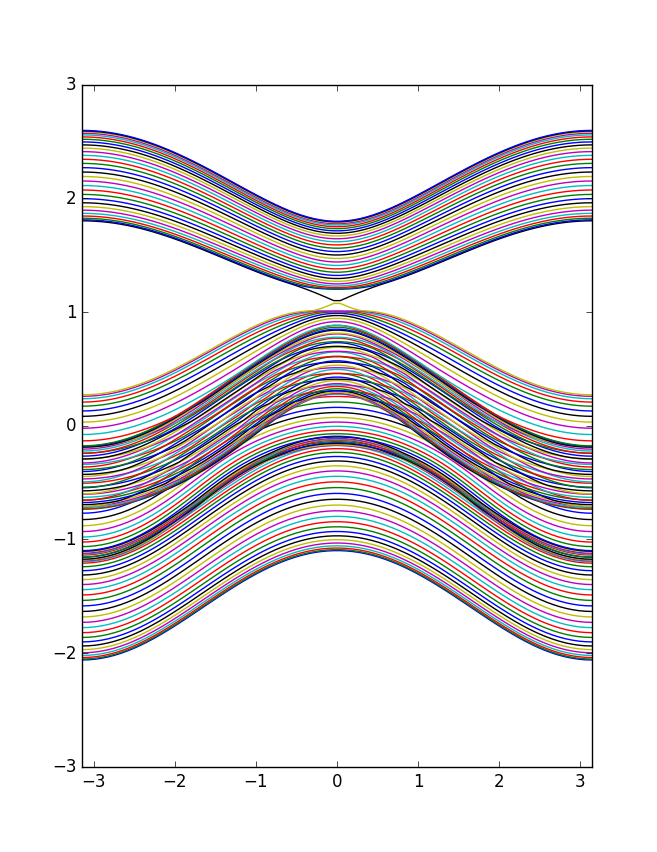
\includegraphics[height=0.9\textheight]{toy_ham_stripe.png}
    \end{figure}
\end{frame}
\begin{frame}
    \frametitle{Примесные уровни в топологическом изоляторе}
    Уровни определяются уравнением
    \begin{equation}    
        \det{\left[\mathbbm{1} - \Delta E \int \frac{d^2 p}{(2\pi)^2} 
                \frac{\omega + \hat{H}}{\omega^2 - E_p^2}\right]} = 1
    \end{equation}
    или
    \begin{equation}
        \label{integrals}
        \left[
        \begin{split}
            &\int \frac{d^2 p}{(2\pi)^2} 
                \frac{\omega + \xi + \frac{1}{m}(2 - \cos{p_x} - \cos{p_y})}
                     {\omega^2 - E_p^2} = \frac{1}{\Delta E},\\
            &\int \frac{d^2 p}{(2\pi)^2} 
                \frac{-\omega + \xi + \frac{1}{m}(2 - \cos{p_x} - \cos{p_y})}
                     {\omega^2 - E_p^2} = -\frac{1}{\Delta E},
        \end{split}
        \right.
    \end{equation}
\end{frame}
\begin{frame}
    \frametitle{Примесные уровни в топологическом изоляторе}
    \begin{columns}
        \begin{column}{0.5\linewidth}
        \begin{figure}[h]
            \centering
            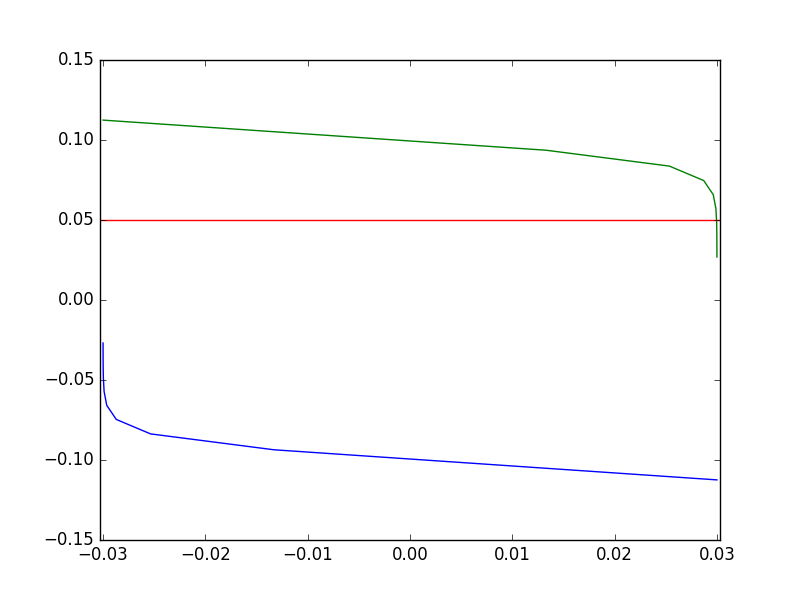
\includegraphics[width=0.95\linewidth]{green_functions.png}
            \caption{$\xi$ < 0}
        \end{figure}
        \end{column}
        \begin{column}{0.5\linewidth}
        \begin{figure}[h]
            \centering
            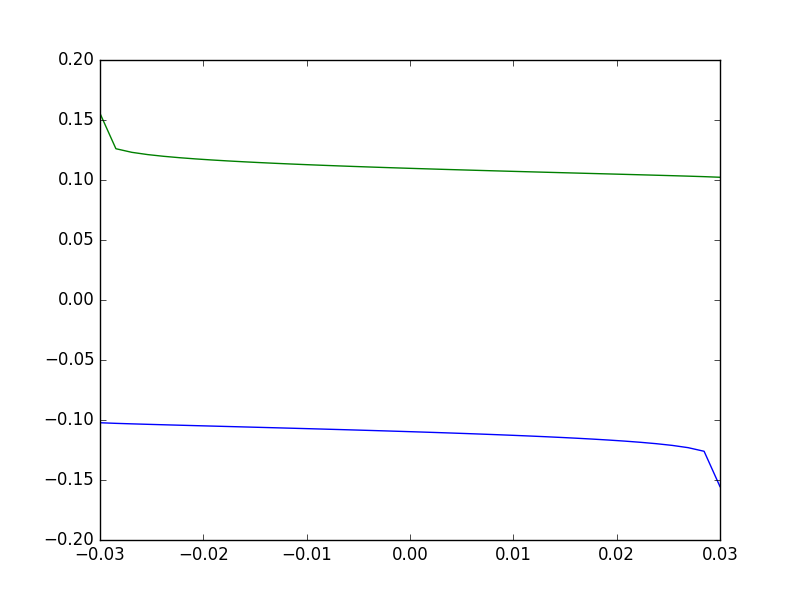
\includegraphics[width=0.95\linewidth]{green_functions_1.png}
            \caption{$\xi$ > 0}
        \end{figure}
        \end{column}
    \end{columns}
\end{frame}
\end{document}
